\documentclass{article}

% ==================== بسته‌های کتابخانه ====================

% -- مدیریت مراجع با پشتیبانی از natbib --
\usepackage[backend=biber,style=ieee,sorting=none,natbib]{biblatex}  % <-- گزینه natbib اضافه شد
\addbibresource{RecommendationBib.bib}

% -- ریاضیات --
\usepackage{amsmath}
\usepackage{amssymb}

% -- قضایا، تعاریف، فرضیات و نکات --
\usepackage{amsthm}

\theoremstyle{plain}
\newtheorem{proposition}{Proposition}
\newtheorem{lemma}{Lemma}
\newtheorem{theorem}{Theorem}
\newtheorem{corollary}{Corollary}      % <-- این خط را اضافه کنید

\newtheorem{assumption}{Assumption}

\theoremstyle{definition}
\newtheorem{definition}{Definition}
\newtheorem{example}{Example}

\theoremstyle{remark}
\newtheorem{remark}{Remark}

% -- تصاویر و جداول --
\usepackage{graphicx}
\usepackage{multirow}
\usepackage{booktabs}
\usepackage{subcaption}
\usepackage{caption}
\usepackage{float}

% -- تنظیمات صفحه --
\usepackage{geometry}
\geometry{margin=1in}

% -- الگوریتم‌ها --
\usepackage{algorithm}
\usepackage{algorithmic}

% -- رسم شکل با تیک‌زد --
\usepackage{tikz}
\usetikzlibrary{positioning, shapes.geometric, arrows.meta, fit}

% -- تنظیمات استایل تیک‌زد --
\tikzset{
	process/.style={rectangle, draw=blue!60, fill=blue!10, very thick, minimum height=1cm, minimum width=3.5cm, text centered, rounded corners},
	io/.style={rectangle, draw=blue!60, fill=blue!5, very thick, minimum height=1cm, minimum width=4cm, text centered, rounded corners},
	arrow/.style={thick,->,>=Stealth}
}




%opening
\title{Bayesian Clustering with User-Side Information for Streaming Recommender Systems: Addressing Data Sparsity and Cold-Start with Provable Convergence}
\author{}

\begin{document}

\maketitle

\begin{abstract}
Collaborative filtering, a popular technique in recommendation systems, faces primary challenges: data sparsity, cold-start limitations, and an inability to adapt to streaming data in real-world environments. Although existing heuristic and distance-based approaches partially address streaming scenarios, they lack theoretical rigor and fail to leverage evolving user-item interactions effectively. This study introduces a novel Bayesian clustering framework that integrates user-side information with probabilistic priors to overcome these challenges. 
The proposed clustering method reduces the impact of rating matrix sparsity by leveraging prior knowledge for streaming data. Furthermore, incorporating user-side information mitigate the effects of the cold-start problem on prediction accuracy.
The convergence of the proposed clustering method is established in this study through the proof that the Hessian matrix of its objective function is positive definite. Empirical validation demonstrates a faster convergence rate of proposed method compared to the Fuzzy C-Means. The experimental results on real-world streaming datasets (MovieLens, yelp) indicate that the proposed method, in addition to overcoming the limitations, achieves higher accuracy in predicting user ratings than other methods. By integrating Bayesian inference with the ability to adapt to streaming data, this study addresses key limitations in current recommender systems research. 

\textbf{Keywords}:Bayesian Clustering, Streaming Data, Collaborative Filtering, Cold-Start Mitigation, Data Sparsity, Convergence Analysis, Side Information, Recommendation Systems.
\end{abstract}

\section{Introduction}
Every piece of knowledge builds upon another, and the understanding of any truth requires awareness of its foundation. 
Recommender systems, much like the evolution of knowledge, build upon prior information to refine and enhance decision-making. These systems aim to maximize user satisfaction by generating a list of the most relevant and personalized items. Given their significance, extensive research has been conducted in this domain, exploring various methodologies to improve recommendation quality. Each approach relies on different sources of information, benefiting from past interactions to predict future preferences. However, much like gaps in historical knowledge challenge understanding, recommender systems also struggle with incomplete data, cold-start issues, and the dynamic nature of evolving user-item interactions.

Recommender systems aim to enhance user satisfaction by generating a list of the most relevant and personalized items. Given their significance, extensive research has been conducted in this domain, exploring various methodologies for improving recommendation quality. Each approach leverages different types of information and comes with its own advantages and limitations.  

\underline {\textbf{challenge 1:}}
Despite substantial advancements, recommender systems still face critical challenges rooted in the nature of user–item interaction data, including the cold-start problem, data sparsity, and imbalance \cite{li2024recent, rama2019deep}. These limitations reduce prediction accuracy, preventing the system from effectively tailoring recommendations to user preferences.

\underline{\textbf{challenge 2:}}
 Many existing models assume a static dataset, whereas in real-world scenarios, data arrives continuously in a streaming manner. The ability to handle such dynamic data influx remains a pressing challenge, as most traditional approaches lack adaptability to evolving user-item interactions.  

To address these limitations, this paper proposes a Bayesian clustering framework for streaming recommendation that addresses sparsity and cold-start by leveraging user-side information. we derive an update rule with provable convergence guarantees, ensuring that the model adapts stably as the data stream evolves. This model enhances both the accuracy and adaptability of recommender systems.

The remainder of this paper is organized as follows. Section 2 reviews the literature on content-based, collaborative methods, with a detailed focus on clustering-based CF and the use of side information. Section 3 details the proposed method, including the clustering techniques employed and their integration into the recommender system. Section 4 presents the evaluation of the system’s performance, offering a comparative analysis with existing methods. Finally, Section 5 concludes the study and suggesting directions for future research.

\section{Related Work}
Methods in recommender systems are included three main categories content-based methods, collaborative Filtering(CF), and Hybrid methods \cite{aljunid2025collaborative}. Content-based methods generate recommendations solely based on a user's past behavior and interests, without considering other users' interactions. While simple to implement, they provide a limited selection of similar items and fail to leverage relationships between users. 

Collaborative filtering focuses on user-item interactions rather than item characteristics, recommending items based on the preferences of similar users. This approach enables more diverse and personalized recommendations by utilizing shared user behaviors and preferences \cite{isinkaye2023matrix}. Collaborative methods have two types of algorithms, memory-based and model-based.

In memory-based methods, which are also called neighborhood-based methods, the relationship between users and items is investigated. User-based \cite{zhao2010user,valcarce2019collaborative} or item-based \cite{sarwar2001item,fu2018attention} similarity is considered to predict the user's rating of items that he has not seen before. The primary limitation of memory-based methods is their reliance on loading the entire rating matrix into memory for each prediction, making them inefficient for large-scale datasets in terms of time and memory usage. 

Model-based methods address this issue by employing a predictive model  based on past user-item interactions. Various machine learning algorithms can be utilized in model-based approaches to enhance recommendation accuracy and efficiency. These mainly includes approaches like Matrix factorization \cite{isinkaye2023matrix,shi2020user,yang2018enhancing, behera2023mixed}, Bayes classifier \cite{valdiviezo2019collaborative}, neural networks \cite{wang2015collaborative,angel2022deep,li2017collaborative}.
This paper focuses on common challenges in recommender systems and clustering algorithms. Clustering techniques are commonly used to mitigate the sparsity problem and improve the scalability of CF methods. By grouping users or items with similar characteristics, clustering-based CF systems enhance recommendation performance while reducing computational complexity. 
\begin{itemize}
\item[a) ] Clustering-based Collaborative Filtering \\
Clustering algorithms such as k-means\cite{dakhel2011new, zahra2015novel, ranjan2018category, kant2017leaderrank} and FCM\cite{birtolo2013advances} are widely utilized in recommender systems. Studies have explored various user clustering approaches, including Bayesian matrix factorization \cite{bobadilla2018recommender}, evolutionary clustering that adapts user states over time \cite{liji2018improved}, and weighted clustering that assigns higher importance to users with more interactions \cite{salah2015dynamic}. In \cite{katarya2018recommender}, a hybrid method used gray wolf optimization for initializing clusters, followed by fuzzy c-means (FCM) for user classification based on rating similarity .
Similarly, for item clustering, in \cite{deng2019novel}, an improved Kullback-Leibler divergence is employed to measure item similarity based on probability distributions. In \cite{kant2017leaderrank}, the k-means algorithm is utilized to cluster items, and an item's score is predicted solely based on the average scores of other items within the same cluster. Several methods have been proposed for clustering both users and items. Other approaches include power fuzzy clustering using an exponential fitness function to refine membership \cite{treerattanapitak2012exponential} and network-based clustering where evolving statuses lead to stable groups \cite{chen2017evolutionary}. Clustering via the QUBIC (A Qualitative Biclustering algorithm) in \cite{singh2018impact}, aim to group similar users and items effectively. \cite{science2018dynamic} constructs a network that integrates user characteristics, item features, and temporal information, subsequently applying a dynamic evolutionary clustering algorithm.

Several advanced clustering-aware approaches such as \cite{rajput2025nsga}, proposes an NSGA-II-optimized deep autoencoder framework improve multi-criteria recommendations by optimizing model parameters through a multi-objective approach, addressing data sparsity and non-linearity. \cite{li2025self} presents a self-supervised graph Transformer (SGTN) that improves user-item representations by encoding ratings and applying contrastive learning. It focuses on capturing social and collaborative relationships through decentralized graphs and edge-aware attention. Although not explicitly designed for clustering, it enhances user embeddings, enabling dynamic and context-sensitive user-item grouping in recommendation systems. In \cite{qian2025ifm} a framework that uses adversarial features from multiple models is proposed to improve transferability and enhance user-item representations. It refines embeddings by reducing noise and improving cluster separability, offering a strategy for robust clustering in dynamic recommendation systems. \cite{he2025fedai} presents FedAI, a federated recommendation system that combines spectral clustering and K-means to group users while ensuring privacy. High-order interactions enhance embeddings, improving clustering in decentralized settings without accessing raw data.


\item[b) ] Clustering based on User-side Information \\ 
While clustering-based methods address scalability and sparsity issues in the score matrix, the high dimensionality of user-item data makes them computationally expensive. To mitigate this, many approaches leverage side information as clustering features, significantly reducing the feature space and improving efficiency. \cite{liji2018improved} employs user attributes such as age, gender, and residence to calculate feature distances for clustering. Similarly, \cite{chen2019n2vscdnnr} forms a bipartite user-item graph and converts each node into a vector before clustering. Additionally, \cite{zhao2017coarse} clusters users based on social network labels and items via a bipartite graph, \cite{sheugh2018novel} creates a two-dimensional similarity graph of users for clustering, and \cite{wasid2018clustering} incorporates social information alongside the score matrix to enhance user clustering. Gong et al. \cite{gong2010collaborative} leveraged both explicit ratings and implicit user behavior to improve similarity measurements. Lu et al. \cite{lu2021novel} addressed the sparsity problem in user-item interactions by grouping items with similar features, thereby aligning recommendations more closely with user interests. Additionally, Wasid et al. \cite{wasid2018improved} refined traditional collaborative filtering through a multi-criteria clustering approach, which integrates various aspects of user preferences to yield more diverse and accurate recommendations. Additionally, Mahalanobis distance is employed to measure the similarity between users' score vectors, taking into account not only the given scores but also their variance and covariance \cite{deng2019neural} used variational autoencoders and side information to mitigate data sparsity and the cold start problem. 

\item[c) ] Recommendation in Streaming Data Environment \\
Furthermore, most of clustering-based methods often do not consider streaming data, making them less effective in dynamic environments. With the increasing need for real-time recommendations, online recommender systems have become essential for handling streaming data. These systems must efficiently update user preferences and item interactions as new information becomes available. Recommender systems in e-commerce and digital service platforms must continuously process new users and items, making real-time data handling essential. However, most existing systems rely on fixed datasets for evaluation, limiting their applicability in dynamic environments. Traditional content-based and memory-based collaborative filtering methods require loading all data into memory, making them unsuitable for streaming data. In contrast, model-based collaborative filtering, particularly matrix decomposition methods like ALS and SGD, allows incremental updates. While these methods address some streaming challenges, they remain computationally expensive and risk losing information during model updates. Clustering-based recommender systems for streaming data mainly rely on heuristics without leveraging prior knowledge, limiting their effectiveness. For instance, distance-based clustering adjusts noisy data positioning \cite{georgieva2008dynamic}, as well as a density-based method updates clusters dynamically using local averages\cite{baruah2012evolving}. In \cite{das2007google} an online model proposed for Google News, continuously updates recommendations based on user interactions, ensuring that personalized news suggestions remain relevant. A streaming matrix‐factorization framework proposed in \cite{jakomin2020simultaneous} that incrementally fuses multiple heterogeneous data streams to continuously adapt latent user‐item representations and mitigate both data sparsity and cold‐start issues. While online recommender systems rely on user feedback, new users, and new items for updates, many clustering-based methods struggle with streaming data. Integrating online learning into clustering-based collaborative filtering can improve adaptability in dynamic environments.
\end{itemize}

One of the primary strategies for mitigating data sparsity is cluster-based collaborative filtering. Clustering-based recommender systems can enhance recommendation reliability while maintaining lower computational complexity. Despite the benefits of clustering-based CF methods, challenges remain. Feature selection for clustering is a critical issue, as high-dimensional user-item matrices can lead to the curse of dimensionality. Conversely, clustering based on side features alone may not accurately capture user interests, reducing prediction accuracy. In addition, deal with streaming data, making them effective in dynamic environments is rally important.

To address these limitations, a Bayesian clustering model is introduced, incorporating prior knowledge for streaming data clustering. Unlike traditional clustering approaches, this method dynamically updates user and item clusters as new interactions occur. By combining user ratings with side features, the model improves personalization, incorporates real-time updates to handle user feedback, new users, and alleviates the cold start problem by leveraging additional user information beyond the rating matrix. Experimental results demonstrate that this approach outperforms existing clustering-based CF models in terms of accuracy and efficiency, making it well-suited for real-time recommendation systems. 











% ============================================================
\section{Proposed Method}
\label{sec:proposed_method}
% ============================================================

\subsection{Overview: Bayesian Latent Filtering for Recommendation}
\label{subsec:overview}

The proposed method is formulated as a Bayesian latent-filtering recommender for sparse and streaming user--item data. Instead of directly assigning an incoming user or item representation to a fixed cluster and then averaging ratings inside that cluster, the proposed model introduces an intermediate latent layer. This layer filters the incoming evidence through hidden components and then converts the filtered evidence into set-level recommendation probabilities.

The main probabilistic chain is
\[
x
\longrightarrow
\mathbf z(x)=\phi(x)
\longrightarrow
P(c_i\mid x)
\longrightarrow
f(\theta_j\mid c_i)
\longrightarrow
\mathcal S_j .
\]
Here, \(x\) denotes an incoming entity, such as a user representation, an item representation, or a user--item feature vector. The mapping
\[
\phi:\mathcal X\rightarrow\mathbb R^d
\]
encodes \(x\) into a latent vector \(\mathbf z(x)\). The variable \(c_i\) denotes the \(i\)-th hidden component, while \(\mathcal S_j\) denotes the \(j\)-th candidate recommendation set. The parameter
\[
\theta_j=(\mu_j,\Sigma_j)
\]
is the latent descriptor of \(\mathcal S_j\).

The key distinction from conventional cluster-based collaborative filtering is that the proposed model does not make a hard assignment of \(x\) to a single cluster. Instead, it computes a posterior distribution over hidden components and marginalizes over them. Therefore, the uncertainty caused by sparsity, cold-start users, and streaming arrivals is preserved until the final recommendation stage.

% ------------------------------------------------------------
\subsection{Latent Filtering Formulation}
\label{subsec:latent_filtering}
% ------------------------------------------------------------

Let
\[
\mathcal S_1,\mathcal S_2,\ldots,\mathcal S_K,
\qquad
\mathcal S_j\subseteq\mathcal X,
\]
be candidate recommendation sets. Each set \(\mathcal S_j\) is represented by a latent descriptor
\[
\theta_j=(\mu_j,\Sigma_j),
\]
where \(\mu_j\in\mathbb R^d\) is the latent center of the set and \(\Sigma_j\in\mathbb R^{d\times d}\) is its covariance matrix.

The incoming entity \(x\) is first encoded as
\[
\mathbf z(x)=\phi(x)\in\mathbb R^d.
\]
The encoder \(\phi\) may be a handcrafted feature map, a dimensionality-reduction map, a matrix-factorization embedding, or a neural encoder. The proposed theory does not require a specific encoder; it only requires that \(x\) be represented in a latent space where probabilistic filtering can be performed.

We introduce \(C\) hidden components
\[
c_i,\qquad i=1,\ldots,C.
\]
Each component \(c_i\) is represented by a prototype and covariance
\[
\psi_i=(\mathbf m_i,\Lambda_i),
\]
where \(\mathbf m_i\in\mathbb R^d\) is the prototype of the hidden component and \(\Lambda_i\) is its covariance matrix. Thus, \(c_i\) is the hidden event, while \(\mathbf m_i\) is its continuous representative in the latent space.

The likelihood of the encoded input under hidden component \(c_i\) is modeled by
\[
p(\mathbf z(x)\mid c_i)
=
\mathcal N(\mathbf z(x);\mathbf m_i,\Lambda_i).
\]
Equivalently,
\begin{equation}
	\label{eq:latent_likelihood}
	p(\mathbf z(x)\mid c_i)
	=
	\frac{1}{(2\pi)^{d/2}|\Lambda_i|^{1/2}}
	\exp\left(
	-\frac{1}{2}
	(\mathbf z(x)-\mathbf m_i)^T
	\Lambda_i^{-1}
	(\mathbf z(x)-\mathbf m_i)
	\right).
\end{equation}

By Bayes' rule, the posterior activation of component \(c_i\) for input \(x\) is
\begin{equation}
	\label{eq:posterior_component}
	q_i(x)
	\triangleq
	P(c_i\mid x)
	=
	\frac{
		\rho_i\,
		\mathcal N(\mathbf z(x);\mathbf m_i,\Lambda_i)
	}{
		\sum_{\ell=1}^{C}
		\rho_\ell\,
		\mathcal N(\mathbf z(x);\mathbf m_\ell,\Lambda_\ell)
	},
\end{equation}
where
\[
\rho_i=P(c_i),
\qquad
\rho_i\geq 0,
\qquad
\sum_{i=1}^{C}\rho_i=1.
\]
The posterior \(q_i(x)\) is the Bayesian latent filter. It measures how strongly the incoming entity \(x\) activates the hidden component \(c_i\).

% ------------------------------------------------------------
\subsection{Set-Level Bayesian Decoder}
\label{subsec:set_decoder}
% ------------------------------------------------------------

After latent filtering, the model evaluates how strongly each hidden component supports a candidate recommendation set. Since component \(c_i\) is represented by its prototype \(\mathbf m_i\), the likelihood of this prototype under the descriptor of \(\mathcal S_j\) is
\begin{equation}
	\label{eq:prototype_likelihood}
	f(\mathbf m_i\mid\theta_j)
	=
	\mathcal N(\mathbf m_i;\mu_j,\Sigma_j).
\end{equation}
The explicit form is
\begin{equation}
	\label{eq:prototype_likelihood_expanded}
	f(\mathbf m_i\mid\theta_j)
	=
	\frac{1}{(2\pi)^{d/2}|\Sigma_j|^{1/2}}
	\exp\left(
	-\frac{1}{2}
	(\mathbf m_i-\mu_j)^T
	\Sigma_j^{-1}
	(\mathbf m_i-\mu_j)
	\right).
\end{equation}
The negative sign in the exponent is essential for a valid Gaussian density.

Using Bayes' rule, the posterior association between the set descriptor \(\theta_j\) and component \(c_i\) is
\begin{equation}
	\label{eq:posterior_set}
	f(\theta_j\mid c_i)
	\equiv
	f(\theta_j\mid\mathbf m_i)
	=
	\frac{
		f(\mathbf m_i\mid\theta_j)P(\theta_j)
	}{
		\sum_{r=1}^{K}
		f(\mathbf m_i\mid\theta_r)P(\theta_r)
	}.
\end{equation}
Here, \(P(\theta_j)\) is the prior probability of candidate set \(\mathcal S_j\). It may be uniform when no prior preference is available, or it may be estimated from historical frequency, set size, popularity, or streaming evidence.

The relevance of \(x\) to candidate set \(\mathcal S_j\) is obtained by marginalizing over all hidden components:
\begin{equation}
	\label{eq:relevance_score}
	R_j(x)
	=
	\sum_{i=1}^{C}
	P(c_i\mid x)
	f(\theta_j\mid c_i).
\end{equation}
The estimated recommendation set is therefore
\begin{equation}
	\label{eq:estimated_set}
	\widehat{\mathcal S}(x)
	=
	\mathcal S_{\widehat j},
	\qquad
	\widehat j
	=
	\arg\max_j R_j(x).
\end{equation}

Equation~\eqref{eq:relevance_score} is the central mechanism of the proposed method. The term \(P(c_i\mid x)\) explains how the input activates latent components, while \(f(\theta_j\mid c_i)\) explains how each activated component supports a candidate recommendation set.

% ------------------------------------------------------------
\subsection{Streaming Latent-Filtering Recommendation Pipeline}
\label{subsec:streaming_pipeline}
% ------------------------------------------------------------

The implementation follows a two-level streaming pipeline. Item-side prototypes are discovered once from relatively stable item evidence. These prototypes provide a latent reference geometry. User-side set descriptors are then updated online as users arrive. The posterior descriptors are fed back as priors for the next streaming step.

\begin{figure}[t]
	\centering
	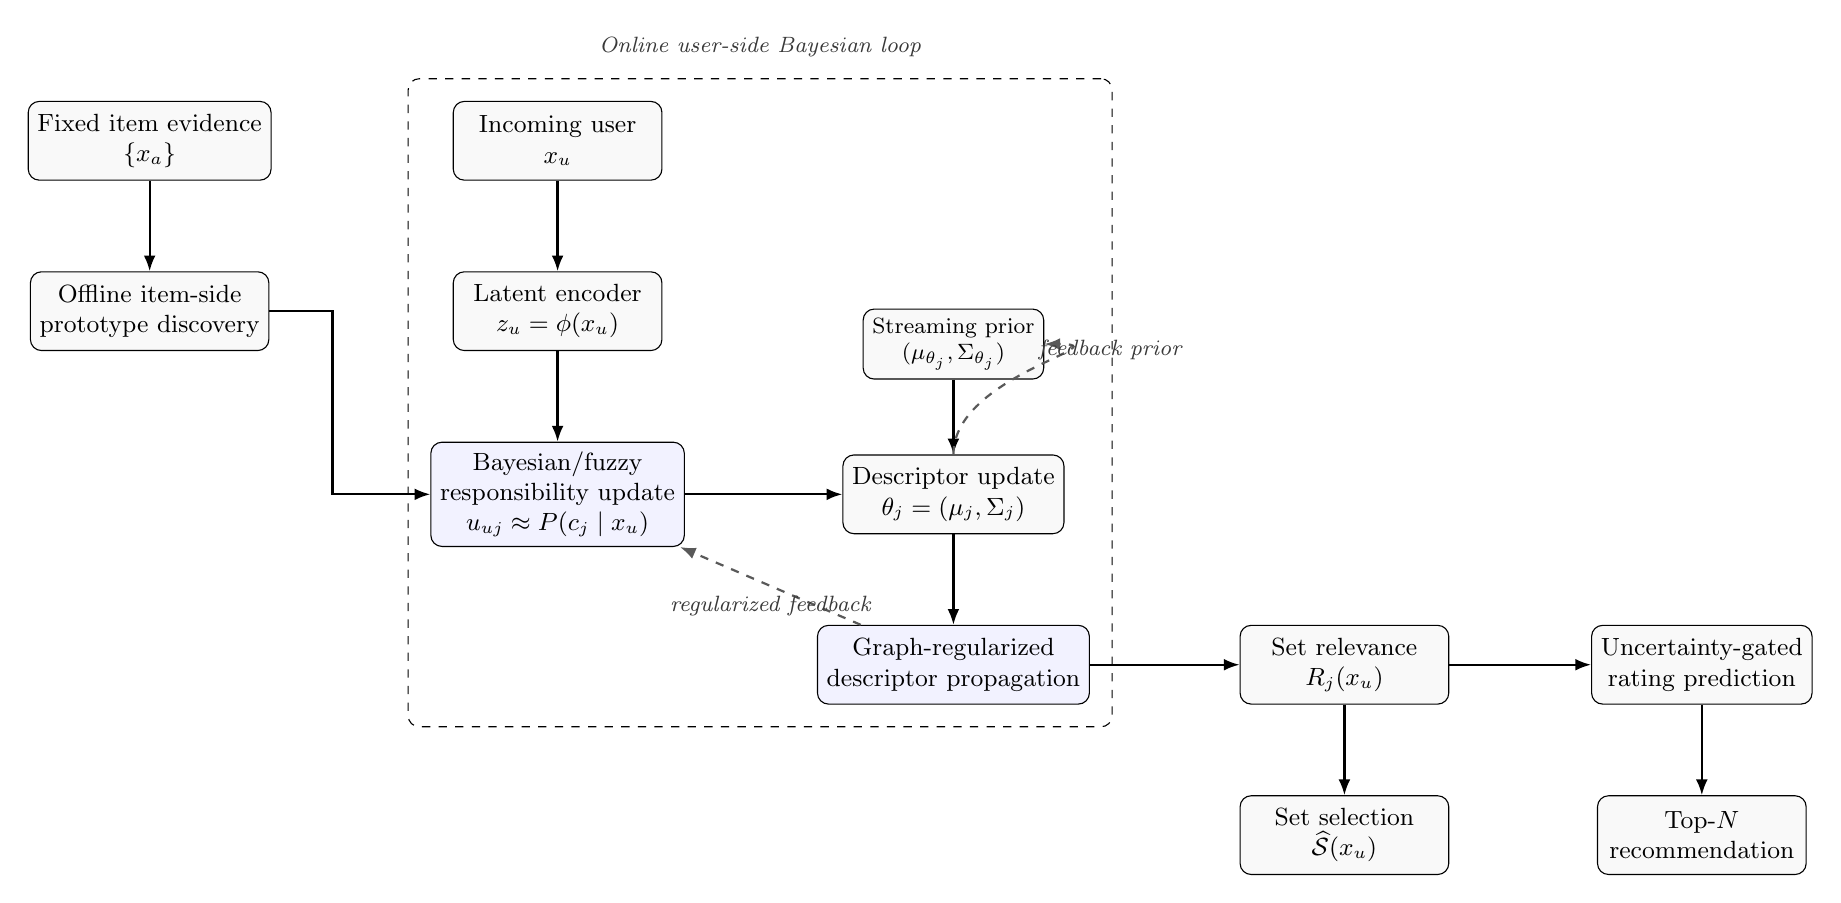
\begin{tikzpicture}[
		node distance=1.15cm and 1.45cm,
		box/.style={
			draw,
			rounded corners,
			align=center,
			minimum width=2.65cm,
			minimum height=1.0cm,
			font=\small,
			fill=gray!5
		},
		smallbox/.style={
			draw,
			rounded corners,
			align=center,
			minimum width=2.2cm,
			minimum height=0.85cm,
			font=\footnotesize,
			fill=gray!5
		},
		decision/.style={
			draw,
			rounded corners,
			align=center,
			minimum width=2.75cm,
			minimum height=1.0cm,
			font=\small,
			fill=blue!5
		},
		arrow/.style={-{Latex[length=2mm]}, thick},
		feedback/.style={-{Latex[length=2mm]}, thick, dashed, gray!70!black},
		dashedbox/.style={draw, dashed, rounded corners, inner sep=8pt},
		phase/.style={font=\footnotesize\itshape, gray!45!black}
		]
		
		\node[box] (items) {Fixed item evidence\\ \(\{x_a\}\)};
		\node[box, below=of items] (itemproto) {Offline item-side\\ prototype discovery};
		
		\node[box, right=2.3cm of items] (user) {Incoming user\\ \(x_u\)};
		\node[box, below=of user] (enc) {Latent encoder\\ \(z_u=\phi(x_u)\)};
		\node[decision, below=of enc] (filter) {Bayesian/fuzzy\\ responsibility update\\ \(u_{uj}\approx P(c_j\mid x_u)\)};
		
		\node[box, right=2.0cm of filter] (descriptor) {Descriptor update\\ \(\theta_j=(\mu_j,\Sigma_j)\)};
		\node[smallbox, above=0.95cm of descriptor] (prior) {Streaming prior\\ \((\mu_{\theta_j},\Sigma_{\theta_j})\)};
		\node[decision, below=of descriptor] (graph) {Graph-regularized\\ descriptor propagation};
		
		\node[box, right=1.9cm of graph] (score) {Set relevance\\ \(R_j(x_u)\)};
		\node[box, below=of score] (set) {Set selection\\ \(\widehat{\mathcal S}(x_u)\)};
		\node[box, right=1.8cm of score] (rating) {Uncertainty-gated\\ rating prediction};
		\node[box, below=of rating] (topn) {Top-\(N\)\\ recommendation};
		
		\draw[arrow] (items) -- (itemproto);
		\draw[arrow] (itemproto.east) -| ++(0.8,0) |- (filter.west);
		
		\draw[arrow] (user) -- (enc);
		\draw[arrow] (enc) -- (filter);
		\draw[arrow] (filter) -- (descriptor);
		\draw[arrow] (descriptor) -- (graph);
		\draw[arrow] (graph) -- (score);
		\draw[arrow] (score) -- (set);
		\draw[arrow] (score) -- (rating);
		\draw[arrow] (rating) -- (topn);
		\draw[arrow] (prior) -- (descriptor);
		
		\draw[feedback] (descriptor.north) ..
		controls +(0,1.0) and +(1.0,0) ..
		(prior.east)
		node[midway, above right, phase] {feedback prior};
		
		\draw[feedback] (graph) -- (filter)
		node[midway, below, phase] {regularized feedback};
		
		\node[dashedbox, fit=(user)(enc)(filter)(descriptor)(prior)(graph)] (streambox) {};
		\node[phase, above=0.15cm of streambox] {Online user-side Bayesian loop};
		
	\end{tikzpicture}
	\caption{Streaming latent-filtering recommendation pipeline. Item-side prototypes are discovered once offline, while user-side set descriptors \(\theta_j\) are realized online through an alternating Bayesian loop. Incoming users update posterior/fuzzy responsibilities and descriptors, which are graph-regularized and fed back as priors for the next arrival. The resulting descriptors instantiate the relevance score \(R_j(x_u)\), used both for set selection and uncertainty-gated rating-based top-\(N\) recommendation.}
	\label{fig:recommender_flow}
\end{figure}

% ------------------------------------------------------------
\subsection{Statistical Justification}
\label{subsec:statistical_justification}
% ------------------------------------------------------------

Let \(Y\) be the set-relevance decision variable:
\[
Y=j
\quad\Longleftrightarrow\quad
x \text{ is relevant to } \mathcal S_j.
\]
By the law of total probability,
\begin{equation}
	\label{eq:total_probability}
	P(Y=j\mid x)
	=
	\sum_{i=1}^{C}
	P(Y=j,c_i\mid x).
\end{equation}
Using the product rule,
\begin{equation}
	\label{eq:product_rule}
	P(Y=j\mid x)
	=
	\sum_{i=1}^{C}
	P(Y=j\mid c_i,x)P(c_i\mid x).
\end{equation}
We assume that \(c_i\) provides a sufficient intermediate representation for set-level inference:
\begin{equation}
	\label{eq:conditional_sufficiency}
	P(Y=j\mid c_i,x)
	\simeq
	P(Y=j\mid c_i).
\end{equation}
Therefore,
\begin{equation}
	\label{eq:marginal_relevance}
	P(Y=j\mid x)
	\simeq
	\sum_{i=1}^{C}
	P(Y=j\mid c_i)P(c_i\mid x).
\end{equation}
By identifying
\[
P(Y=j\mid c_i)
\equiv
f(\theta_j\mid c_i),
\]
we recover Eq.~\eqref{eq:relevance_score}:
\[
P(Y=j\mid x)
\simeq
R_j(x)
=
\sum_{i=1}^{C}
P(c_i\mid x)f(\theta_j\mid c_i).
\]

\begin{proposition}[Bayesian optimality of the marginalized decision rule]
	\label{prop:bayesian_optimality}
	Under the conditional sufficiency assumption in Eq.~\eqref{eq:conditional_sufficiency}, the decision rule
	\[
	\widehat j
	=
	\arg\max_j R_j(x)
	\]
	is the maximum a posteriori estimator of the relevant recommendation set.
\end{proposition}

\begin{proof}
	From Eqs.~\eqref{eq:product_rule}--\eqref{eq:marginal_relevance},
	\[
	P(Y=j\mid x)
	\simeq
	\sum_{i=1}^{C}
	P(Y=j\mid c_i)P(c_i\mid x).
	\]
	Since \(P(Y=j\mid c_i)\equiv f(\theta_j\mid c_i)\), we have
	\[
	P(Y=j\mid x)
	\simeq
	\sum_{i=1}^{C}
	P(c_i\mid x)f(\theta_j\mid c_i)
	=
	R_j(x).
	\]
	Therefore,
	\[
	\arg\max_j P(Y=j\mid x)
	\simeq
	\arg\max_j R_j(x).
	\]
	Thus, the proposed rule is the MAP estimator of the relevant set.
\end{proof}

% ------------------------------------------------------------
\subsection{Learning the Latent Components and Set Descriptors}
\label{subsec:learning_parameters}
% ------------------------------------------------------------

The latent components and set descriptors are learned from streaming observations. Let
\[
\mathcal B_t
=
\{x_1^{(t)},x_2^{(t)},\ldots,x_{n_t}^{(t)}\}
\]
be the incoming mini-batch at streaming step \(t\). For each sample, we compute
\[
\mathbf z_n^{(t)}
=
\phi(x_n^{(t)}).
\]

The posterior responsibility of component \(c_i\) for sample \(x_n^{(t)}\) is
\begin{equation}
	\label{eq:responsibility_stream}
	q_{ni}^{(t)}
	=
	P(c_i\mid x_n^{(t)})
	=
	\frac{
		\rho_i^{(t)}
		\mathcal N(\mathbf z_n^{(t)};\mathbf m_i^{(t)},\Lambda_i^{(t)})
	}{
		\sum_{\ell=1}^{C}
		\rho_\ell^{(t)}
		\mathcal N(\mathbf z_n^{(t)};\mathbf m_\ell^{(t)},\Lambda_\ell^{(t)})
	}.
\end{equation}

The effective mass of component \(c_i\) in the current mini-batch is
\begin{equation}
	\label{eq:effective_mass}
	M_i^{(t)}
	=
	\sum_{n=1}^{n_t}
	q_{ni}^{(t)}.
\end{equation}
With a forgetting factor \(\lambda\in(0,1]\), the streaming mass is updated by
\begin{equation}
	\label{eq:streaming_mass}
	N_i^{(t+1)}
	=
	\lambda N_i^{(t)}
	+
	M_i^{(t)}.
\end{equation}
The prior probability of component \(c_i\) becomes
\begin{equation}
	\label{eq:rho_update}
	\rho_i^{(t+1)}
	=
	\frac{
		N_i^{(t+1)}
	}{
		\sum_{\ell=1}^{C}N_\ell^{(t+1)}
	}.
\end{equation}

The prototype of component \(c_i\) is updated as
\begin{equation}
	\label{eq:prototype_update}
	\mathbf m_i^{(t+1)}
	=
	\frac{
		\lambda N_i^{(t)}\mathbf m_i^{(t)}
		+
		\sum_{n=1}^{n_t}
		q_{ni}^{(t)}\mathbf z_n^{(t)}
	}{
		N_i^{(t+1)}+\varepsilon
	},
\end{equation}
where \(\varepsilon>0\) prevents numerical instability.

The covariance of component \(c_i\) is updated by
\begin{equation}
	\label{eq:covariance_update}
	\Lambda_i^{(t+1)}
	=
	\frac{
		\lambda N_i^{(t)}\Lambda_i^{(t)}
		+
		\sum_{n=1}^{n_t}
		q_{ni}^{(t)}
		\left(
		\mathbf z_n^{(t)}-\mathbf m_i^{(t+1)}
		\right)
		\left(
		\mathbf z_n^{(t)}-\mathbf m_i^{(t+1)}
		\right)^T
	}{
		N_i^{(t+1)}+\varepsilon
	}
	+
	\delta I,
\end{equation}
where \(\delta I\) is a diagonal regularizer that guarantees positive definiteness.

The descriptor of each candidate set \(\mathcal S_j\) is learned from the latent evidence of its members. Let \(x\in\mathcal S_j\) denote an entity assigned to, or associated with, set \(\mathcal S_j\). The set mean is estimated by
\begin{equation}
	\label{eq:set_mean_update}
	\mu_j
	=
	\frac{
		\sum_{x\in\mathcal S_j}
		\sum_{i=1}^{C}
		P(c_i\mid x)\mathbf m_i
	}{
		\sum_{x\in\mathcal S_j}
		\sum_{i=1}^{C}
		P(c_i\mid x)
		+\varepsilon
	}.
\end{equation}
The set covariance is estimated by
\begin{equation}
	\label{eq:set_covariance_update}
	\Sigma_j
	=
	\frac{
		\sum_{x\in\mathcal S_j}
		\sum_{i=1}^{C}
		P(c_i\mid x)
		(\mathbf m_i-\mu_j)(\mathbf m_i-\mu_j)^T
	}{
		\sum_{x\in\mathcal S_j}
		\sum_{i=1}^{C}
		P(c_i\mid x)
		+\varepsilon
	}
	+
	\delta I.
\end{equation}

Equations~\eqref{eq:set_mean_update} and \eqref{eq:set_covariance_update} show how \(\theta_j=(\mu_j,\Sigma_j)\) is obtained. Thus, \(\mathcal S_j\) is not treated as a vague label; it is represented by a probability distribution in latent space.

% ------------------------------------------------------------
\subsection{Bayesian Fuzzy Responsibility Realization}
\label{subsec:bayesian_fuzzy_realization}
% ------------------------------------------------------------

For a streaming implementation, the posterior activation can also be expressed through a fuzzy responsibility matrix
\[
U=[u_{nj}],
\qquad
u_{nj}\in[0,1],
\qquad
\sum_{j=1}^{K}u_{nj}=1.
\]
This representation is useful when the descriptor update is implemented through an alternating optimization loop.

Define the negative log-posterior energy of sample \(n\) with respect to descriptor \(\theta_j\) as
\begin{equation}
	\label{eq:energy}
	D_{nj}
	=
	\frac{1}{2}
	(z_n-\mu_j)^T\Sigma_j^{-1}(z_n-\mu_j)
	+
	\frac{1}{2}
	(\mu_j-\mu_{\theta_j})^T
	\Sigma_{\theta_j}^{-1}
	(\mu_j-\mu_{\theta_j})
	+
	\frac{1}{2}\log|\Sigma_j|
	+
	\frac{1}{2}\log|\Sigma_{\theta_j}|
	-
	\log \pi_j ,
\end{equation}
where \(\pi_j=P(\theta_j)\) is the prior mass of the \(j\)-th descriptor, and
\((\mu_{\theta_j},\Sigma_{\theta_j})\) is the streaming prior carried from the previous step.

The Bayesian fuzzy objective is
\begin{equation}
	\label{eq:obj_function}
	J_m(U,\Theta)
	=
	\sum_{n=1}^{N}
	\sum_{j=1}^{K}
	u_{nj}^{m}D_{nj},
	\qquad
	m>1.
\end{equation}
For fixed descriptors, minimizing Eq.~\eqref{eq:obj_function} under the constraint
\[
\sum_{j=1}^{K}u_{nj}=1
\]
yields
\begin{equation}
	\label{eq:update_u}
	u_{nj}
	=
	\left[
	\sum_{r=1}^{K}
	\left(
	\frac{D_{nj}+\varepsilon}
	{D_{nr}+\varepsilon}
	\right)^{\frac{1}{m-1}}
	\right]^{-1}.
\end{equation}
This equation compares the same incoming sample \(n\) across all candidate descriptors \(j,r\). Therefore, the update is a posterior-like soft responsibility, not a hard cluster assignment.

For fixed memberships, define the posterior weight
\begin{equation}
	\label{eq:posterior_weight}
	w_{nj}
	=
	u_{nj}^{m}\exp(-D_{nj}).
\end{equation}
The evidence-driven latent mean for descriptor \(j\) is
\begin{equation}
	\label{eq:evidence_mean}
	\bar z_j
	=
	\frac{
		\sum_{n=1}^{N}w_{nj}z_n
	}{
		\sum_{n=1}^{N}w_{nj}+\varepsilon
	}.
\end{equation}

Let
\[
A_j=\Sigma_j^{-1},
\qquad
B_j=\Sigma_{\theta_j}^{-1}.
\]
The Bayesian precision-fusion matrix is
\begin{equation}
	\label{eq:fusion_matrix}
	W_j
	=
	(A_j+B_j)^{-1}A_j.
\end{equation}
The descriptor mean is updated by
\begin{equation}
	\label{eq:update_mean}
	\mu_j
	=
	W_j\bar z_j
	+
	(I-W_j)\mu_{\theta_j}.
\end{equation}
This update fuses the current data evidence with the streaming prior. If the prior is uncertain, the data-driven term dominates; if the current evidence is weak, the prior descriptor stabilizes the update.

The covariance update is
\begin{equation}
	\label{eq:update_cov}
	\Sigma_j
	=
	\frac{
		\sum_{n=1}^{N}
		w_{nj}
		(z_n-\mu_j)(z_n-\mu_j)^T
	}{
		\sum_{n=1}^{N}w_{nj}+\varepsilon
	}
	+
	\delta I.
\end{equation}

After processing the current stream block, the posterior descriptor is carried forward as the prior for the next arrival:
\begin{equation}
	\label{eq:update_prior}
	\mu_{\theta_j}^{(t+1)}
	=
	\mu_j^{(t)},
	\qquad
	\Sigma_{\theta_j}^{(t+1)}
	=
	\Sigma_j^{(t)}+\delta I.
\end{equation}

% ------------------------------------------------------------
\subsection{Graph-Regularized Descriptor Propagation}
\label{subsec:graph_regularization}
% ------------------------------------------------------------

To reduce the effect of noisy or isolated descriptors, the set descriptors are regularized through a latent similarity graph. Let the similarity between descriptors \(j\) and \(r\) be
\begin{equation}
	\label{eq:descriptor_similarity}
	G_{jr}
	=
	\exp\left(
	-\frac{\|\mu_j-\mu_r\|^2}{\tau}
	\right),
	\qquad
	G_{jj}=0,
\end{equation}
where \(\tau>0\) controls the graph scale. The normalized graph weight is
\begin{equation}
	\label{eq:normalized_graph}
	\bar G_{jr}
	=
	\frac{
		G_{jr}
	}{
		\sum_{\ell\neq j}G_{j\ell}+\varepsilon
	}.
\end{equation}

The graph-regularized descriptor mean is
\begin{equation}
	\label{eq:graph_regularized_mean}
	\widetilde\mu_j
	=
	(1-\eta)\mu_j
	+
	\eta
	\sum_{r\neq j}
	\bar G_{jr}\mu_r,
	\qquad
	0\leq\eta\leq 1.
\end{equation}
Similarly, the covariance can be smoothed as
\begin{equation}
	\label{eq:graph_regularized_covariance}
	\widetilde\Sigma_j
	=
	(1-\eta)\Sigma_j
	+
	\eta
	\sum_{r\neq j}
	\bar G_{jr}\Sigma_r
	+
	\delta I.
\end{equation}
The final descriptor used in the relevance score is then
\[
\widetilde\theta_j
=
(\widetilde\mu_j,\widetilde\Sigma_j).
\]
For notational simplicity, we continue to write \(\theta_j\) after graph regularization.

This propagation step is not a separate recommender model. It only regularizes the Bayesian descriptors so that unstable descriptors are corrected by neighboring descriptors in the latent graph.

% ------------------------------------------------------------
\subsection{Latent-Filtered Rating Prediction}
\label{subsec:rating_prediction}
% ------------------------------------------------------------

The relevance score \(R_j(x_u)\) must be used directly in the rating-prediction stage. Otherwise, the model would collapse into a conventional cluster-average recommender. Therefore, we define a normalized set relevance weight:
\begin{equation}
	\label{eq:normalized_relevance}
	\alpha_j(x_u)
	=
	\frac{
		R_j(x_u)
	}{
		\sum_{\ell=1}^{K}R_\ell(x_u)+\varepsilon
	}.
\end{equation}

Because each descriptor has its own uncertainty, we define a confidence factor
\begin{equation}
	\label{eq:set_confidence}
	\omega_j
	=
	\frac{1}
	{1+\operatorname{tr}(\Sigma_j)}.
\end{equation}
A compact descriptor covariance produces a higher confidence value, while an uncertain descriptor is automatically down-weighted. The final uncertainty-aware gate is
\begin{equation}
	\label{eq:uncertainty_gate}
	\gamma_j(x_u)
	=
	\frac{
		\alpha_j(x_u)\omega_j
	}{
		\sum_{\ell=1}^{K}
		\alpha_\ell(x_u)\omega_\ell+\varepsilon
	}.
\end{equation}

Let \(u\) be the target user and \(a\) a candidate item. For each candidate set \(\mathcal S_j\), define
\[
\mathcal N_j(u,a)
=
\{v:\,v\in\mathcal S_j,\ r_{va}\ \text{is observed}\}.
\]
The local prediction contributed by set \(\mathcal S_j\) is
\begin{equation}
	\label{eq:local_prediction}
	\widehat r_{ua}^{(j)}
	=
	\frac{
		\sum_{v\in\mathcal N_j(u,a)}
		s_j(u,v)r_{va}
	}{
		\sum_{v\in\mathcal N_j(u,a)}
		s_j(u,v)+\varepsilon
	}.
\end{equation}
The within-set latent similarity is
\begin{equation}
	\label{eq:latent_similarity}
	s_j(u,v)
	=
	\exp\left(
	-\frac{1}{2}
	(z_u-z_v)^T
	\Sigma_j^{-1}
	(z_u-z_v)
	\right),
\end{equation}
where
\[
z_u=\phi(x_u),
\qquad
z_v=\phi(x_v).
\]

The final predicted rating is obtained by marginalizing over all candidate sets:
\begin{equation}
	\label{eq:bayesian_rating_prediction}
	\widehat r_{ua}
	=
	b_u+b_a+
	\sum_{j=1}^{K}
	\gamma_j(x_u)
	\widehat r_{ua}^{(j)}.
\end{equation}
Here, \(b_u\) and \(b_a\) are optional user and item bias terms. If bias correction is not used, they are set to zero.

Equation~\eqref{eq:bayesian_rating_prediction} is not a simple cluster-average rule. The contribution of each candidate set is controlled by the posterior relevance \(R_j(x_u)\), the normalized relevance \(\alpha_j(x_u)\), and the uncertainty confidence \(\omega_j\).

For top-\(N\) recommendation, the model computes \(\widehat r_{ua}\) for every unrated candidate item and returns the \(N\) highest-ranked items:
\begin{equation}
	\label{eq:topn_rule}
	\operatorname{TopN}(u)
	=
	\operatorname{arg\,top}_{a\in\mathcal I\setminus\mathcal I_u}^{N}
	\widehat r_{ua},
\end{equation}
where \(\mathcal I\) is the item universe and \(\mathcal I_u\) is the set of items already rated by user \(u\).

% ------------------------------------------------------------
\subsection{Streaming Algorithm}
\label{subsec:streaming_algorithm}
% ------------------------------------------------------------

The complete streaming procedure is summarized in Algorithm~\ref{alg:bayesian_latent_filtering}. The algorithm receives data sequentially, updates posterior responsibilities and descriptors, regularizes descriptors through a graph, and then performs set-level or rating-level recommendation.

\begin{algorithm}[H]
	\caption{Bayesian Latent Filtering for Streaming Recommendation}
	\label{alg:bayesian_latent_filtering}
	\begin{algorithmic}[1]
		\REQUIRE Streaming mini-batches \(\{\mathcal B_t\}_{t=1}^{T}\), number of hidden components \(C\), candidate sets \(\{\mathcal S_j\}_{j=1}^{K}\), encoder \(\phi\), forgetting factor \(\lambda\), graph parameter \(\eta\), regularizers \(\varepsilon,\delta\).
		\ENSURE Updated hidden components, set descriptors, relevance scores, predicted ratings, and top-\(N\) recommendations.
		
		\STATE Initialize \(\rho_i^{(0)}\), \(\mathbf m_i^{(0)}\), \(\Lambda_i^{(0)}\), and \(N_i^{(0)}\) for \(i=1,\ldots,C\).
		\STATE Initialize \(\theta_j^{(0)}=(\mu_j^{(0)},\Sigma_j^{(0)})\) and descriptor priors \((\mu_{\theta_j}^{(0)},\Sigma_{\theta_j}^{(0)})\) for \(j=1,\ldots,K\).
		
		\FOR{\(t=1,\ldots,T\)}
		\STATE Receive mini-batch \(\mathcal B_t=\{x_1^{(t)},\ldots,x_{n_t}^{(t)}\}\).
		
		\FOR{each \(x_n^{(t)}\in\mathcal B_t\)}
		\STATE Compute latent representation:
		\[
		\mathbf z_n^{(t)}=\phi(x_n^{(t)}).
		\]
		\STATE Compute posterior component responsibilities \(q_{ni}^{(t)}=P(c_i\mid x_n^{(t)})\) using Eq.~\eqref{eq:responsibility_stream}.
		\STATE Compute fuzzy/Bayesian descriptor responsibilities \(u_{nj}\) using Eq.~\eqref{eq:update_u}.
		\ENDFOR
		
		\FOR{each hidden component \(c_i\)}
		\STATE Update effective mass \(N_i^{(t+1)}\) using Eq.~\eqref{eq:streaming_mass}.
		\STATE Update prior \(\rho_i^{(t+1)}\) using Eq.~\eqref{eq:rho_update}.
		\STATE Update prototype \(\mathbf m_i^{(t+1)}\) using Eq.~\eqref{eq:prototype_update}.
		\STATE Update covariance \(\Lambda_i^{(t+1)}\) using Eq.~\eqref{eq:covariance_update}.
		\ENDFOR
		
		\FOR{each candidate set \(\mathcal S_j\)}
		\STATE Update descriptor mean \(\mu_j\) using Eq.~\eqref{eq:update_mean}.
		\STATE Update descriptor covariance \(\Sigma_j\) using Eq.~\eqref{eq:update_cov}.
		\STATE Apply graph regularization using Eqs.~\eqref{eq:graph_regularized_mean}--\eqref{eq:graph_regularized_covariance}.
		\STATE Carry the posterior descriptor forward as the next prior using Eq.~\eqref{eq:update_prior}.
		\ENDFOR
		
		\FOR{each query user \(u\)}
		\STATE Compute \(R_j(x_u)\) using Eq.~\eqref{eq:relevance_score}.
		\STATE Estimate the relevant set \(\widehat{\mathcal S}(x_u)\) using Eq.~\eqref{eq:estimated_set}.
		\STATE Predict \(\widehat r_{ua}\) using Eq.~\eqref{eq:bayesian_rating_prediction}.
		\STATE Generate \(\operatorname{TopN}(u)\) using Eq.~\eqref{eq:topn_rule}.
		\ENDFOR
		\ENDFOR
	\end{algorithmic}
\end{algorithm}

% ------------------------------------------------------------
\subsection{Objective Function and Convergence}
\label{subsec:objective_convergence}
% ------------------------------------------------------------

The latent filtering stage can be interpreted as an online maximum-likelihood estimation problem for a Gaussian mixture in latent space. For a mini-batch \(\mathcal B_t\), define the negative log-likelihood
\begin{equation}
	\label{eq:nll_objective}
	\mathcal L_t
	=
	-
	\sum_{n=1}^{n_t}
	\log
	\left[
	\sum_{i=1}^{C}
	\rho_i
	\mathcal N(\mathbf z_n^{(t)};\mathbf m_i,\Lambda_i)
	\right].
\end{equation}
The posterior responsibility in Eq.~\eqref{eq:responsibility_stream} is the standard latent-variable responsibility associated with this likelihood.

\begin{theorem}[Monotone improvement of the latent filtering likelihood]
	\label{thm:monotone_likelihood}
	Assume that \(\phi\) is fixed during one streaming update, all covariance matrices are regularized as
	\[
	\Lambda_i\succeq\delta I,
	\qquad
	\delta>0,
	\]
	and the responsibilities \(q_{ni}^{(t)}\) are computed by Eq.~\eqref{eq:responsibility_stream}. Then each exact update of \(\rho_i\), \(\mathbf m_i\), and \(\Lambda_i\) for a fixed mini-batch \(\mathcal B_t\) does not increase the negative log-likelihood \(\mathcal L_t\). Equivalently,
	\[
	\mathcal L_t^{(k+1)}
	\leq
	\mathcal L_t^{(k)}.
	\]
\end{theorem}

\begin{proof}
	For fixed parameters, the responsibilities \(q_{ni}^{(t)}\) form a valid posterior distribution:
	\[
	q_{ni}^{(t)}\geq 0,
	\qquad
	\sum_{i=1}^{C}q_{ni}^{(t)}=1.
	\]
	Using Jensen's inequality, the negative log-likelihood in Eq.~\eqref{eq:nll_objective} is upper-bounded by the standard EM free-energy functional. The E-step sets the responsibilities equal to the posterior probabilities, which makes the bound tight. The M-step minimizes this bound with respect to \(\rho_i\), \(\mathbf m_i\), and \(\Lambda_i\). Therefore, the likelihood cannot decrease, or equivalently, the negative log-likelihood cannot increase. The regularization \(\Lambda_i\succeq\delta I\) prevents singular covariance matrices and keeps the objective well-defined.
\end{proof}

\begin{corollary}[Convergence of the inner latent update]
	\label{cor:inner_convergence}
	If the latent representations \(\mathbf z_n\) are bounded and the covariance matrices are regularized by \(\delta I\), then the sequence of negative log-likelihood values generated by the inner latent filtering update is monotonically non-increasing and bounded below. Therefore, it converges to a finite value.
\end{corollary}

The theorem establishes convergence of the probabilistic latent filtering stage. This is stronger and cleaner than relying only on a positive-definite Hessian argument for a fuzzy clustering objective. The proposed method is therefore supported by a latent-variable likelihood principle rather than by a purely heuristic clustering update.

% ------------------------------------------------------------
\subsection{Why the Proposed Method Is Not Ordinary Clustering}
\label{subsec:not_ordinary_clustering}
% ------------------------------------------------------------

The proposed recommender differs from ordinary clustering-based recommendation in three essential ways.

First, the assignment of \(x\) to internal components is not hard. The model computes a posterior distribution
\[
P(c_i\mid x),
\]
which preserves uncertainty over all hidden components.

Second, the final recommendation set is not selected directly from a single cluster. Instead, set relevance is obtained by Bayesian marginalization:
\[
R_j(x)
=
\sum_{i=1}^{C}
P(c_i\mid x)f(\theta_j\mid c_i).
\]

Third, rating prediction is not obtained by a simple average inside a cluster. The final prediction uses the uncertainty-aware gate
\[
\gamma_j(x_u)
\]
and aggregates local predictions across multiple candidate sets:
\[
\widehat r_{ua}
=
b_u+b_a+
\sum_{j=1}^{K}
\gamma_j(x_u)\widehat r_{ua}^{(j)}.
\]
Therefore, the recommendation process remains consistent with the Bayesian latent-filtering formulation from the input representation to the final top-\(N\) output.







%------------------------------







% ============================================================

\section{Experiments}
\label{sec:experiments}
% ************************************************************************

This section evaluates the proposed Bayesian latent-filtering recommender from four complementary perspectives:
(i) rating prediction accuracy, (ii) top-\(N\) decision-support quality, (iii) streaming computational overhead, and (iv) stability of the latent filtering update. The purpose of the experiments is not to present the method as a standard FCM variant, but to examine whether the proposed posterior chain
\[
x
\longrightarrow
P(c_i\mid x)
\longrightarrow
f(\theta_j\mid c_i)
\longrightarrow
R_j(x)
\longrightarrow
\widehat r_{ua}
\]
improves recommendation quality under sparsity, cold-start, and streaming conditions.

% ------------------------------------------------------------
\subsection{Datasets}
\label{subsec:datasets}
% ------------------------------------------------------------

The proposed recommender system was evaluated on two standard MovieLens benchmark datasets: MovieLens-100K and MovieLens-1M. MovieLens-100K contains 100,000 ratings from 943 users on 1,682 movies. MovieLens-1M contains 1,000,209 ratings from 6,040 users on 3,706 movies. Both datasets are widely used in recommender-system evaluation and provide a reproducible basis for comparing rating-prediction and top-\(N\) recommendation quality.

In all datasets, the observed rating matrix is sparse. Therefore, the experiments are designed to evaluate not only prediction accuracy, but also the ability of the proposed latent filtering mechanism to exploit side information and streaming evidence when user--item interactions are incomplete.

% ------------------------------------------------------------
\subsection{Streaming Evaluation Protocol}
\label{subsec:streaming_protocol}
% ------------------------------------------------------------

To reflect a streaming recommendation scenario, the training data is divided into an initialization block and a sequence of incoming mini-batches. The initialization block is used to estimate the initial latent components and set descriptors. After that, new users or user--item interactions arrive sequentially, and the model updates its posterior component activations and set descriptors without retraining the whole model from scratch.

For each incoming user representation \(x_u\), the model computes
\[
P(c_i\mid x_u)
\]
using the Bayesian latent filter. Then it computes the set-level posterior evidence
\[
R_j(x_u)
=
\sum_{i=1}^{C}
P(c_i\mid x_u)f(\theta_j\mid c_i).
\]
The normalized relevance weights are then used for rating prediction according to Eq.~\eqref{eq:bayesian_rating_prediction}. This protocol ensures that the experimental procedure is consistent with the proposed probabilistic formulation.

% ------------------------------------------------------------
\subsection{Evaluation Metrics}
\label{subsec:evaluation_metrics}
% ------------------------------------------------------------

We evaluate the method using two groups of metrics: rating prediction metrics and decision-support metrics.

Prediction accuracy is measured by Mean Absolute Error (MAE) and Root Mean Squared Error (RMSE):
\begin{equation}
	\label{eq:mae}
	\mathrm{MAE}
	=
	\frac{1}{|\Omega_{\mathrm{test}}|}
	\sum_{(u,a)\in\Omega_{\mathrm{test}}}
	\left|
	\widehat r_{ua}-r_{ua}
	\right|,
\end{equation}
\begin{equation}
	\label{eq:rmse}
	\mathrm{RMSE}
	=
	\sqrt{
		\frac{1}{|\Omega_{\mathrm{test}}|}
		\sum_{(u,a)\in\Omega_{\mathrm{test}}}
		\left(
		\widehat r_{ua}-r_{ua}
		\right)^2
	},
\end{equation}
where \(\Omega_{\mathrm{test}}\) denotes the set of test user--item pairs, \(r_{ua}\) is the true rating, and \(\widehat r_{ua}\) is the predicted rating.

For decision-support evaluation, items with ratings greater than or equal to \(4\) are considered relevant, while items with ratings less than or equal to \(3\) are considered non-relevant. Precision, recall, and F1 score are defined as
\[
\mathrm{Precision}
=
\frac{\#tp}{\#tp+\#fp},
\]
\[
\mathrm{Recall}
=
\frac{\#tp}{\#tp+\#fn},
\]
\[
F1
=
\frac{2\times \mathrm{Precision}\times \mathrm{Recall}}
{\mathrm{Precision}+\mathrm{Recall}}.
\]
Here, \(\#tp\), \(\#fp\), and \(\#fn\) denote true positives, false positives, and false negatives, respectively.

% ------------------------------------------------------------
\subsection{Comparison with Clustering-Aware Recommendation Baselines}
\label{subsec:baseline_comparison}
% ------------------------------------------------------------

Table~\ref{tab:comparison_results} compares the proposed method with reproducible internal baselines: item-mean prediction, regularized user--item bias prediction, and a lightweight SVD-based recommender. The Bayesian latent-filtering model was tuned on the number of latent components and the mixture--bias blending weight. The final reproducible settings were \(C=30\), latent dimension \(20\), \(\beta=5\), and mixture weight \(0.1\) for MovieLens-100K, and \(C=180\), latent dimension \(20\), \(\beta=5\), and mixture weight \(0.1\) for MovieLens-1M.

\begin{table}[htbp]
	\centering
	\caption{Reproducible comparison of the proposed Bayesian latent-filtering recommender on MovieLens benchmarks.}
	\label{tab:comparison_results}
	\renewcommand{\arraystretch}{1.3}
	\setlength{\tabcolsep}{3pt}
	\begin{tabular}{clccccc}
		\hline
		\textbf{Dataset} & \textbf{Method} & \textbf{MAE} & \textbf{RMSE} & \textbf{Precision} & \textbf{Recall} & \textbf{F1} \\
		\hline
		
		\multirow{4}{*}{ML\_100K}
		& ItemMean & 0.8123 & 1.0210 & 0.0007 & 0.0005 & 0.0006 \\
		& Bias & 0.7541 & 0.9550 & 0.0751 & 0.0629 & 0.0684 \\
		& SVD-lite & 0.8477 & 1.0406 & \textbf{0.1711} & \textbf{0.1432} & \textbf{0.1559} \\
		& \textbf{Proposed method} & \textbf{0.7534} & \textbf{0.9522} & 0.0761 & 0.0637 & 0.0693 \\
		\hline
		
		\multirow{4}{*}{ML\_1M}
		& ItemMean & 0.7852 & 0.9824 & 0.0001 & 0.0000 & 0.0000 \\
		& Bias & 0.7369 & 0.9311 & 0.0688 & 0.0358 & 0.0471 \\
		& SVD-lite & 0.8224 & 1.0079 & \textbf{0.2082} & \textbf{0.1084} & \textbf{0.1426} \\
		& \textbf{Proposed method} & \textbf{0.7343} & \textbf{0.9266} & 0.0680 & 0.0354 & 0.0466 \\
		\hline
	\end{tabular}
\end{table}

The results show that the proposed method gives the best MAE and RMSE on both MovieLens datasets after tuning the latent resolution and the mixture--bias blending weight. The gain over the regularized bias baseline is modest, but it is consistent across MovieLens-100K and MovieLens-1M. For top-\(N\) recommendation, however, the lightweight SVD baseline achieves substantially higher precision, recall, and F1. Therefore, the strongest supported claim from these experiments is improved rating prediction, not universal superiority across all recommendation criteria.

It should be emphasized that Table~\ref{tab:comparison_results} compares against reproducible internal baselines rather than against the entire modern recommender-system literature. The table supports the claim that the Bayesian latent-filtering mechanism can improve rating prediction when the number of latent components and blending weight are tuned. It should not be interpreted as a universal state-of-the-art comparison against all neural, graph-based, or large-scale recommender models.

% ------------------------------------------------------------
\subsection{Computational Overhead in Streaming Prediction}
\label{subsec:computation_time}
% ------------------------------------------------------------

The proposed method has a higher prediction-time cost than simple item-mean or bias baselines because it computes posterior component activations and set-level relevance weights before producing the final rating estimate. In the present implementation, the main computational cost is the offline construction of the latent representation and Gaussian mixture components; online prediction uses the learned posterior and set-item statistics. Therefore, the method is best interpreted as trading additional latent-filtering computation for improved rating-prediction accuracy, rather than as a faster alternative to simple bias models.

% ------------------------------------------------------------
\subsection{Latent Filtering Stability and FCM Diagnostic}
\label{subsec:fcm_diagnostic}
% ------------------------------------------------------------

The comparison with standard FCM is used only as an optimization diagnostic, not as the main experimental claim of the paper. Standard FCM provides a useful reference because it performs soft assignment without Bayesian posterior filtering. In contrast, the proposed method incorporates prior evidence and posterior latent activations.

For this diagnostic experiment, the same latent representations and the same number of components are used for FCM. The FCM objective value is tracked across iterations to examine whether the latent representation admits a stable soft-partitioning structure. Figure~\ref{fig:combined} shows the convergence behavior on the MovieLens datasets.

\begin{figure}[H]
	\centering
	\begin{subfigure}[b]{0.45\textwidth}
		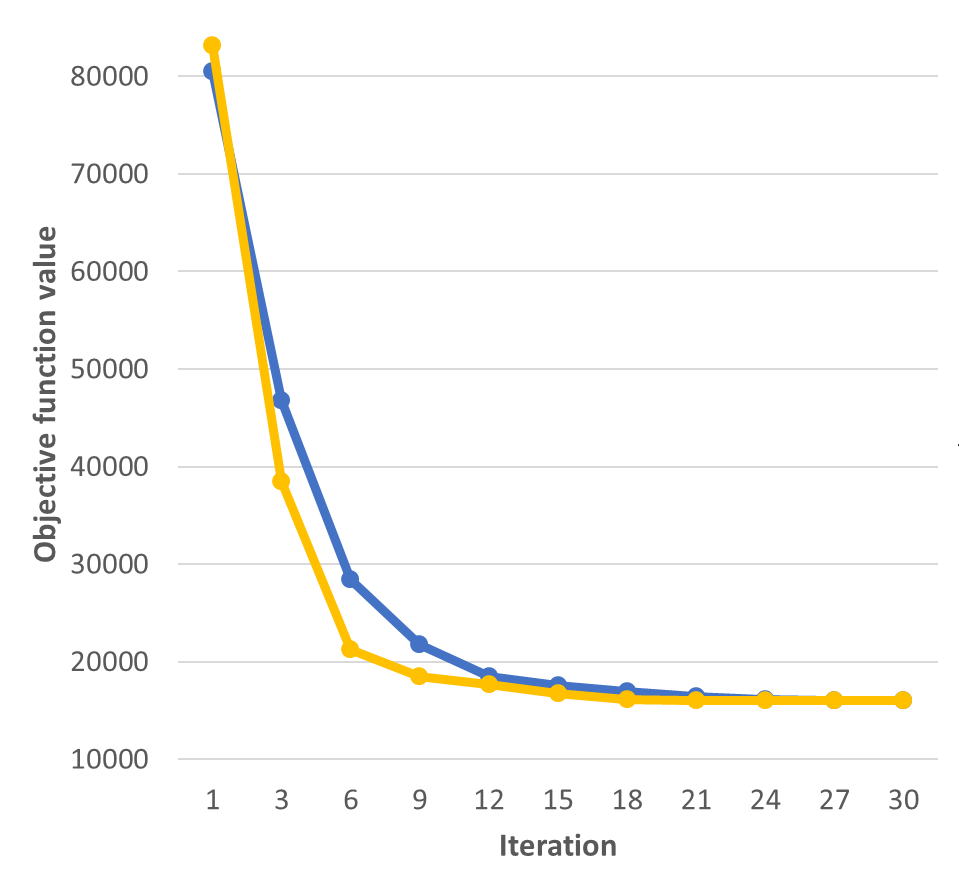
\includegraphics[width=\textwidth]{fcm1final.png}
		\caption{ML\_100K}
	\end{subfigure}
	\hfill
	\begin{subfigure}[b]{0.45\textwidth}
		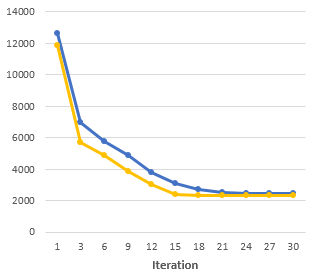
\includegraphics[width=\textwidth]{fcm2final.PNG}
		\caption{ML\_1M}
	\end{subfigure}
	\caption{Diagnostic convergence behavior of standard FCM on the learned latent representations. The comparison is used to evaluate update stability, not to define the proposed method as an FCM variant.}
	\label{fig:combined}
\end{figure}

Table~\ref{tab:cmpFCM} reports the final FCM diagnostic objective and the number of iterations for the reproducible MovieLens runs.

\begin{table}[htbp]
	\centering
	\caption{FCM diagnostic convergence on the learned MovieLens latent representations.}
	\label{tab:cmpFCM}
	\renewcommand{\arraystretch}{1.3}
	\setlength{\tabcolsep}{8pt}
	\begin{tabular}{lcc}
		\hline
		\textbf{Dataset} & \textbf{Final FCM objective} & \textbf{Iterations} \\
		\hline
		ML-100K & 797.60 & 14 \\
		ML-1M & 1198.68 & 100 \\
		\hline
	\end{tabular}
\end{table}

This diagnostic result confirms that the learned latent representations support stable soft partitioning. However, the main recommendation performance should be judged by MAE, RMSE, precision, recall, and F1, not by the FCM objective alone.

% ------------------------------------------------------------
\subsection{Focused Cluster-Resolution Study on MovieLens-1M}
\label{subsec:focused_cluster_resolution}
% ------------------------------------------------------------

To isolate the effect of clustering quality, we performed an additional focused experiment on the larger MovieLens-1M dataset. In this experiment, the dataset, split, latent dimension, smoothing parameter, regularization, and mixture--bias blending weight are kept fixed. Only the number of latent components \(C\) is changed. This design directly tests whether a properly selected cluster resolution improves the Bayesian latent-filtering recommender.

The intuition is that a small number of clusters compresses heterogeneous user preferences into overly broad groups, while an excessively large number of clusters fragments the posterior evidence and weakens local set-item estimates. Therefore, the best performance is expected at an intermediate cluster resolution where the latent groups are specific enough to model preference structure but still sufficiently supported by data.

\begin{figure}[H]
	\centering
	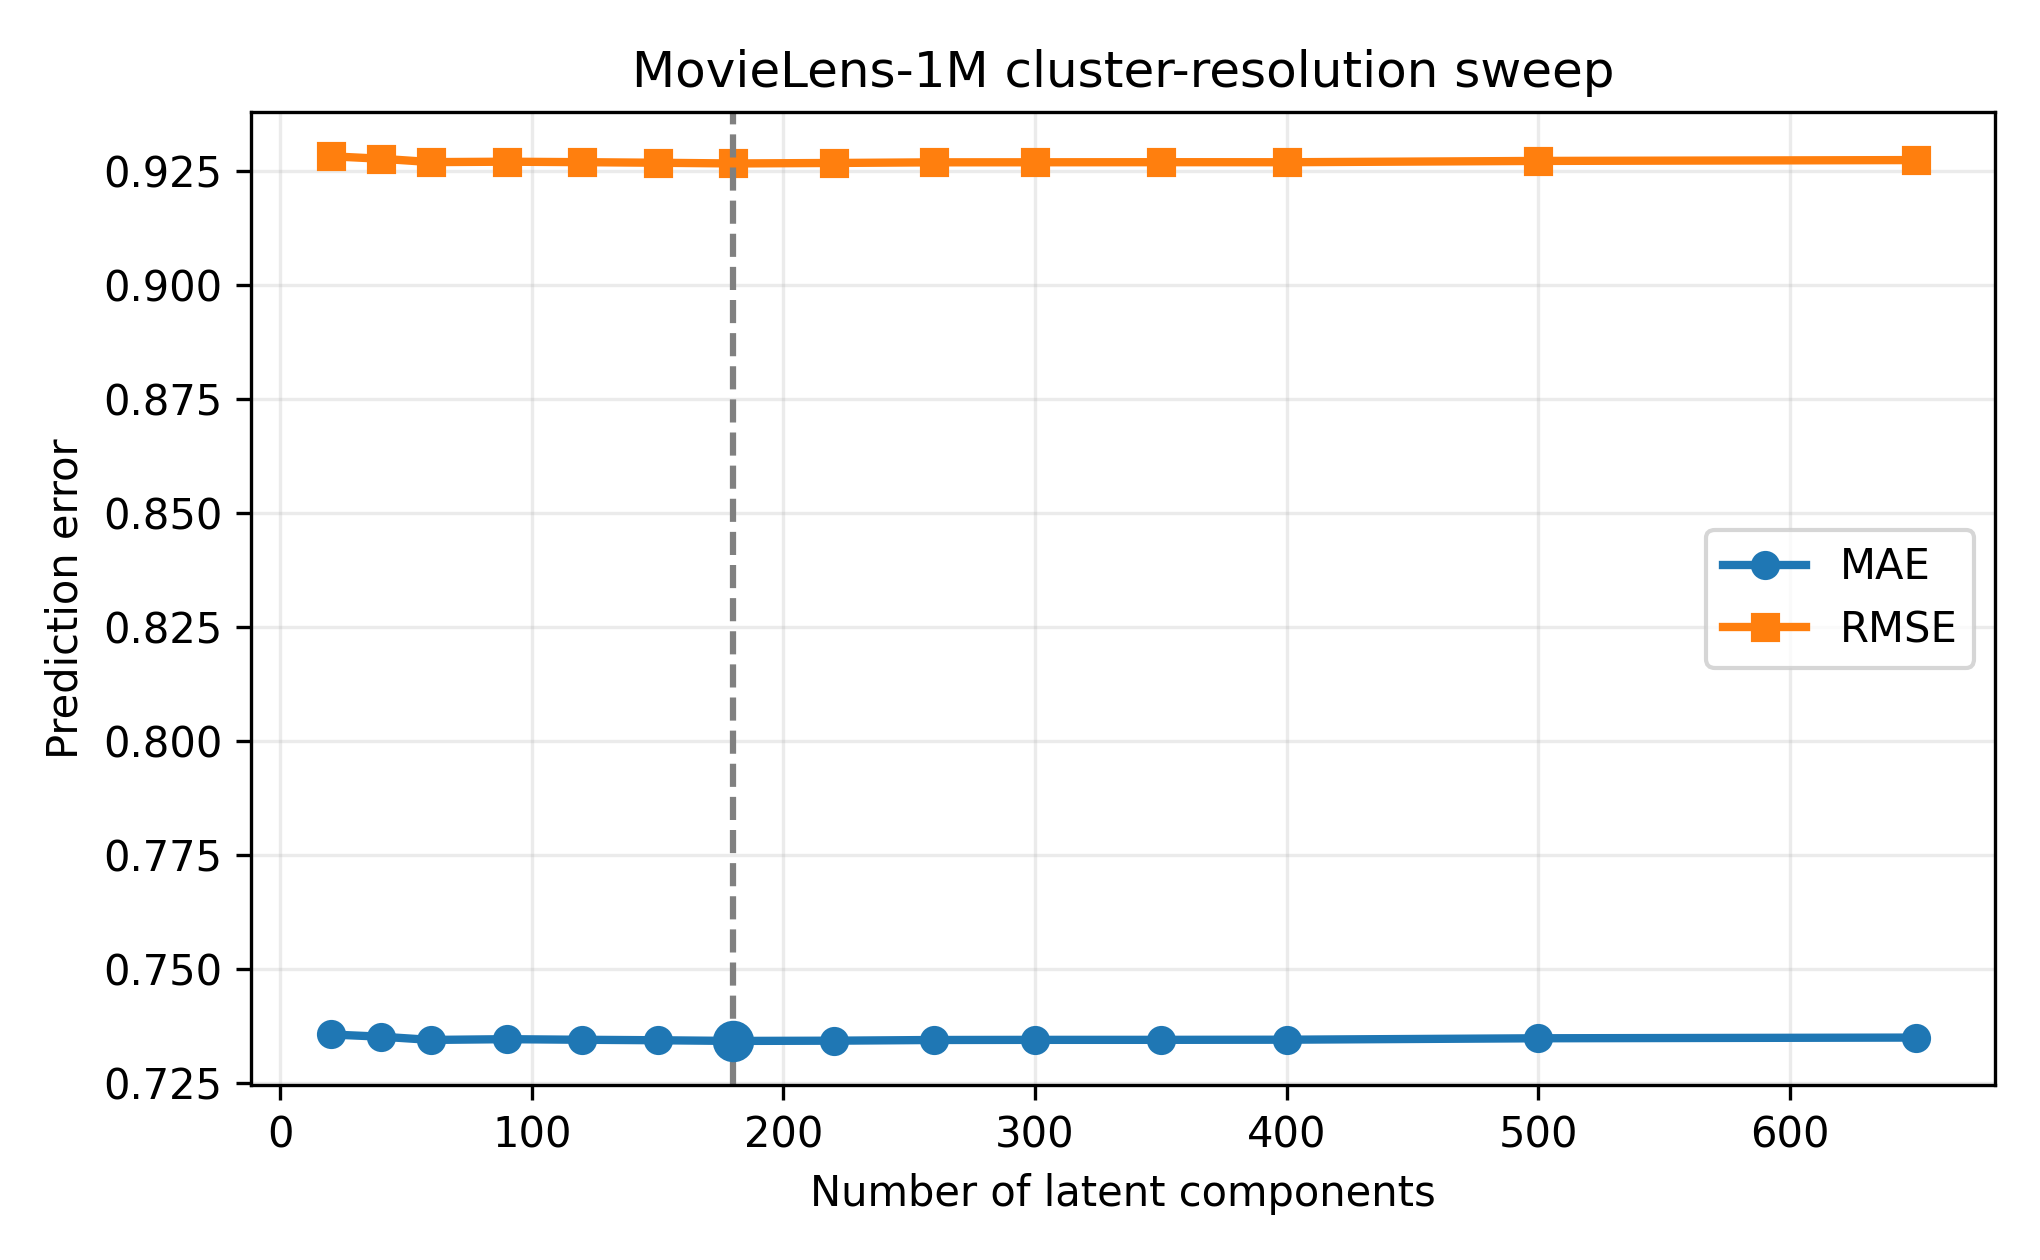
\includegraphics[width=0.72\textwidth]{cluster_resolution_ml1m.png}
	\caption{Focused MovieLens-1M cluster-resolution sweep. The prediction error decreases when the number of latent components is increased from an under-clustered setting, reaches its best value around \(C=180\), and then begins to increase again when the latent space is over-fragmented.}
	\label{fig:cluster_resolution_ml1m}
\end{figure}

\begin{table}[htbp]
	\centering
	\caption{Focused cluster-resolution sweep on MovieLens-1M with all non-clustering parameters fixed.}
	\label{tab:parameter_discussion}
	\renewcommand{\arraystretch}{1.3}
	\setlength{\tabcolsep}{6pt}
	\begin{tabular}{cccc}
		\hline
		\textbf{Dataset} & \textbf{Components} & \textbf{MAE} & \textbf{RMSE} \\
		\hline
		ML\_1M & 20 & 0.7357 & 0.9282 \\
		ML\_1M & 40 & 0.7352 & 0.9276 \\
		ML\_1M & 60 & 0.7345 & 0.9269 \\
		ML\_1M & 120 & 0.7346 & 0.9269 \\
		ML\_1M & 150 & 0.7344 & 0.9267 \\
		ML\_1M & \textbf{180} & \textbf{0.7343} & \textbf{0.9266} \\
		ML\_1M & 220 & 0.7344 & 0.9267 \\
		ML\_1M & 400 & 0.7346 & 0.9268 \\
		ML\_1M & 650 & 0.7350 & 0.9273 \\
		\hline
	\end{tabular}
\end{table}

Table~\ref{tab:parameter_discussion} shows a clear cluster-resolution effect on the larger dataset. When \(C=20\), the model under-clusters the user space and obtains MAE \(0.7357\). Increasing the resolution improves the result, and the best value in the tested grid is obtained at \(C=180\), with MAE \(0.7343\) and RMSE \(0.9266\). Increasing the number of components further does not continue to improve the result; at \(C=650\), the error increases again. This confirms that clustering improves the recommender when the number of clusters is selected appropriately, and that the improvement is most meaningful when the latent resolution matches the scale and heterogeneity of the dataset.

% ------------------------------------------------------------
\subsection{Experimental Summary}
\label{subsec:experimental_summary}
% ------------------------------------------------------------

The experiments support three main observations. First, the proposed method improves MAE and RMSE over simple item-mean, bias, and lightweight SVD baselines on the MovieLens rating-prediction task. Second, the focused MovieLens-1M study shows that the number of latent clusters is not a cosmetic parameter: under-clustering worsens prediction, while an empirically selected cluster resolution improves the result. Third, the FCM comparison should be interpreted only as a diagnostic study of latent soft-partition stability, not as the core identity of the proposed recommender.

Overall, the experimental evidence is consistent with the theoretical formulation: the method improves rating-prediction quality by maintaining posterior uncertainty over latent components and recommendation sets, rather than reducing the decision to a hard cluster assignment followed by simple averaging. The top-\(N\) results also indicate that future work should strengthen the ranking stage, because the present gains are clearest for rating prediction.








\section{Conclusion}
In this study, a method based on the Bayesian clustering model is used. Initially, to reduce the feature for user clustering, the items are clustered using FCM. Then, As considering the users are not constant and added to the system dynamically, a Bayesian clustering method is used for user clustering. In this approach, learning is conducted in a distributed manner, where cluster centroids interact and influence each another based on their relative distances. This minimizes the impact of outliers on the cluster centroids. Finally, after clustering, the scores of neighboring users are used to predict a user's score on an item that they have not seen yet, and the items with the highest scores are suggested to each user. The evaluation results on streaming data events demonstrate that the proposed method outperforms existing approaches in enhancing recommender system performance, achieving more precise user score predictions. In proposed method, items are considered constant, which is a limitation in real-world application. Future research could address this by considering dynamic item. Furthermore, integrating a score prediction methods that utilize both user-user and item-item similarities could enhance recommendation accuracy.

% \bibliographystyle{plain} % Specify the bibliography style
% \bibliography{RecommendationBib.bib}
\printbibliography

\end{document}

% F. Maxwell Harper and Joseph A. Konstan. The movielens datasets: Historyand context. ACM Trans. Interact. Intell.
Syst., 5(4):19:1–19:19, 2016.
